\chapter{Solution design}

\section{Overview}

TODO

\section{Mapping}

In this section we are going to go through the visual mapping part of my thesis.

\subsection{Experimenting with OAK-D}

To begin exploring the capabilities of the camera, I initiated my efforts by testing the example software provided by the camera's manufacturer, namely DepthAI Viewer\footnote{\url{https://github.com/luxonis/depthai-viewer}}. This software proved invaluable for its ability to showcase the camera's functionalities effectively.

Upon installation, I gained access to a user-friendly interface that allowed me to view images captured by the camera in real-time. Additionally, the software facilitated real-time 3D reconstruction of the camera's surroundings, as depicted in Figure \ref{fig:DAI_3d}. Notably, the DepthAI Viewer leveraged the Vision Processing Unit (VPU) embedded within the device, thereby enabling comprehensive exploration of its capabilities, as illustrated in the top left corner of Figure \ref{fig:DAI_person_detection}.

\begin{figure}[H]
	\centering
	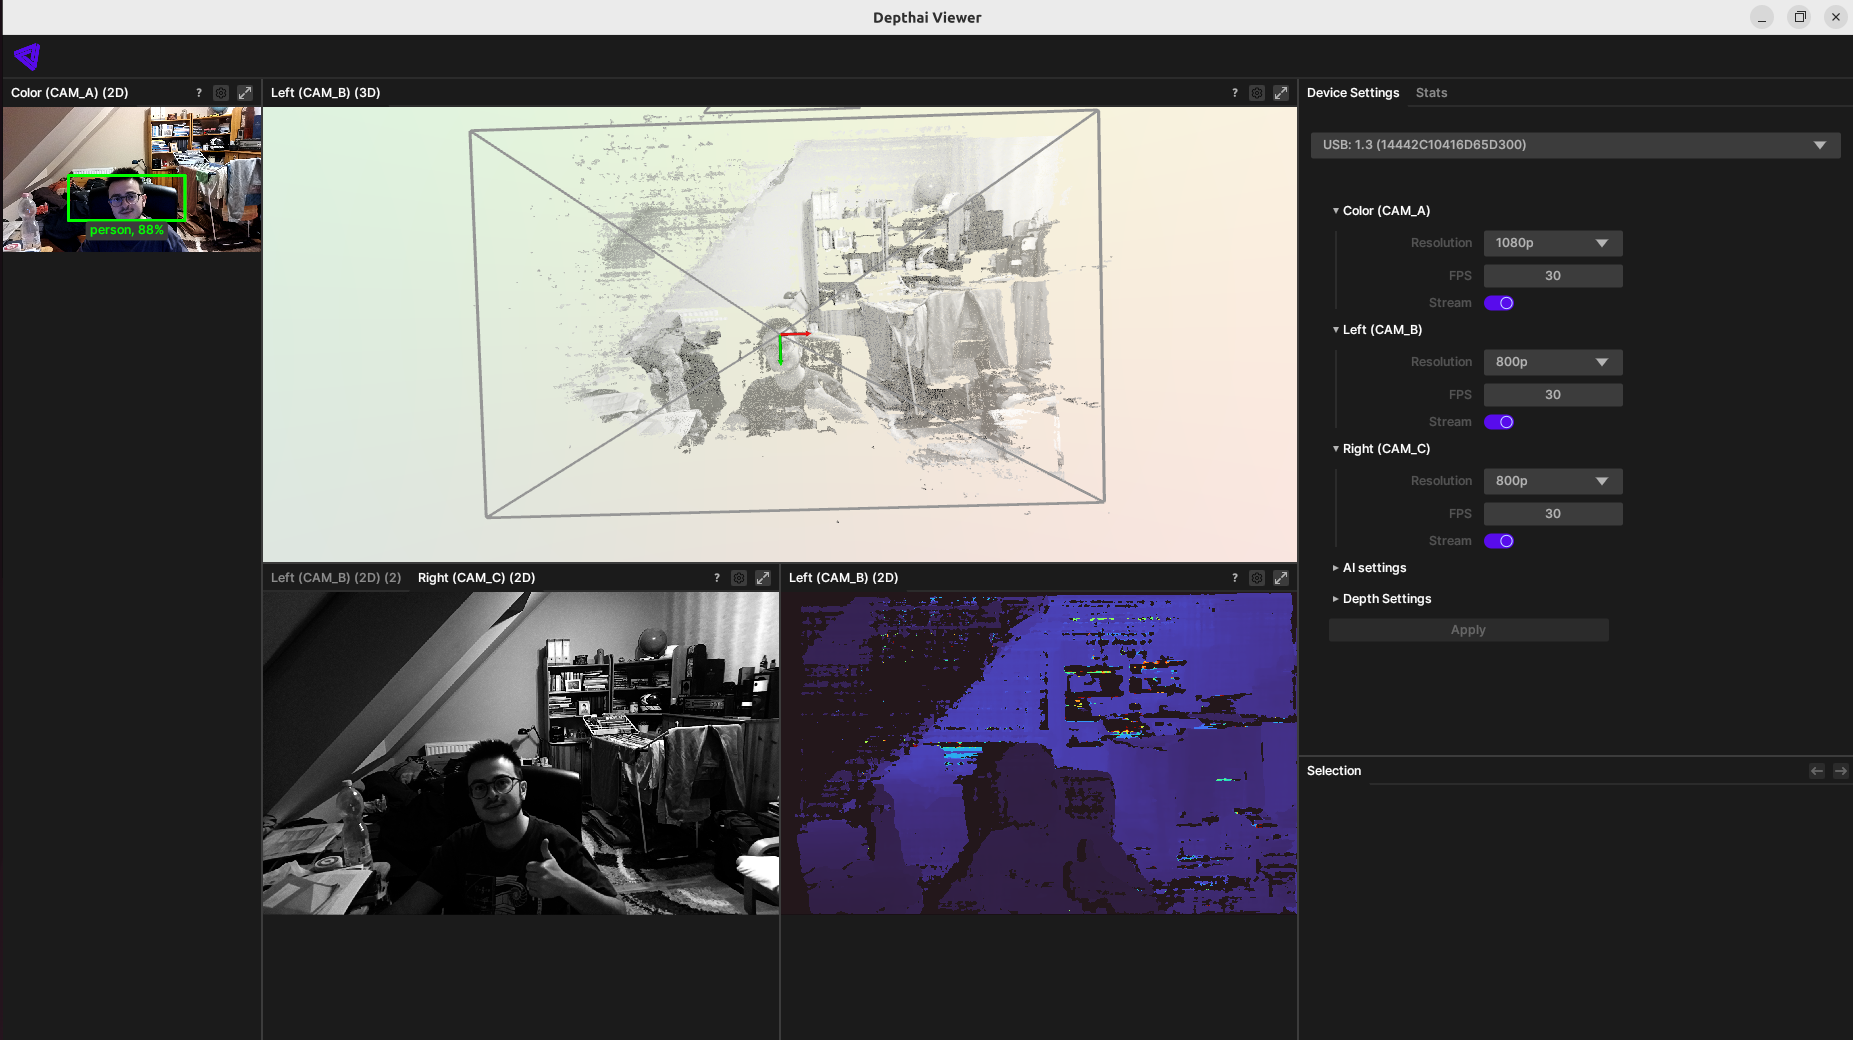
\includegraphics[width=150mm, keepaspectratio]{figures/depthai_viewer.png}
	\caption{DepthAI Viewer with person detection}
	\label{fig:DAI_person_detection}
\end{figure}

\begin{figure}[H]
	\centering
	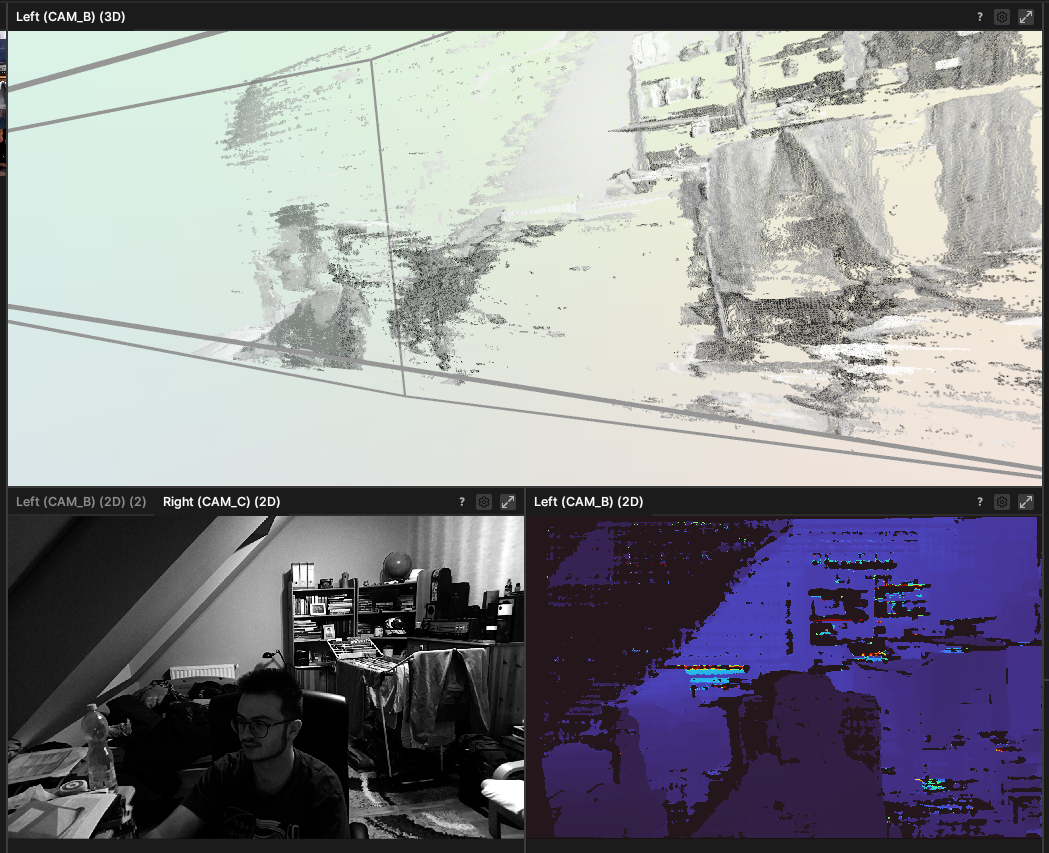
\includegraphics[width=150mm, keepaspectratio]{figures/depthai_viewer_3d.png}
	\caption{DepthAI Viewer's 3D reconstruction}
	\label{fig:DAI_3d}
\end{figure}

This initial exploration served as a foundational step in understanding the camera's capabilities and paved the way for further experimentation and development in subsequent tasks.

The next step was to experiment with the Spectacular AI SDK's examples to determine if it is capable of mapping and detecting persons with low latency. At first the Python scripts threw a warning and they did not work: 
\begin{lstlisting}[language=bash,frame=single,float=!ht]
SpectacularAI WARN: Dropping frames!
SpectacularAI WARN: VIO may be running too slow, data is being input too fast, or IMU samples are missing / time-offset from frames. (buffer size 10)
\end{lstlisting}\\
After some research I found out that this problem is related to outdated firmware version on the camera (note that it took a long time to find the solution due to the severe lack of documentation). To solve the issue, Luxonis' \verb|depthai-python| repo\footnote{\url{https://github.com/luxonis/depthai-python}} must be cloned and the IMU firmware update script\footnote{\url{https://github.com/luxonis/depthai-python/blob/main/examples/IMU/imu_firmware_update.py}} must be ran. After the successful firmware update I was able to try out the examples.

The most simple is the one that visualizes the camera's movement. It extracts the data from the IMU and uses matplotlib for visualization. As we can see on Figure \ref{fig:IMU_visu}, I was able to draw a heart in the air. The curves are not perfect because my hand was probably shaking a bit.

\begin{figure}[H]
	\centering
	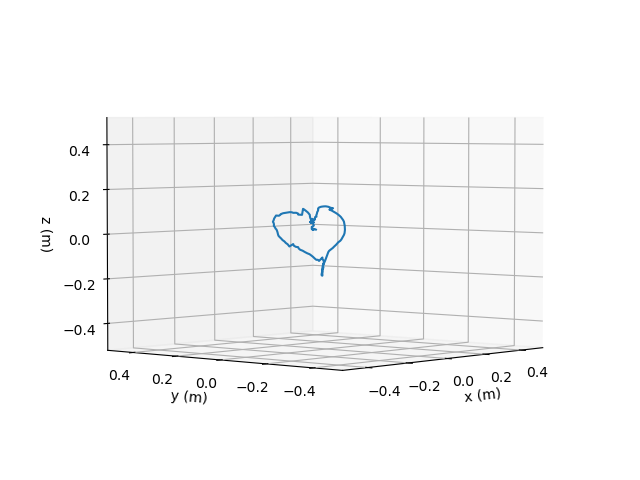
\includegraphics[width=150mm, keepaspectratio]{figures/spectacular_ai_vio_visu.png}
	\caption{IMU visualization with Spectacular AI}
	\label{fig:IMU_visu}
\end{figure}

A bit more advanced example uses the camera too, not just the IMU. When the camera is covered with our hand it visualizes the device's movement with the help of the IMU as we can see on Figure \ref{fig:3d_pen}.

\begin{figure}[H]
	\centering
	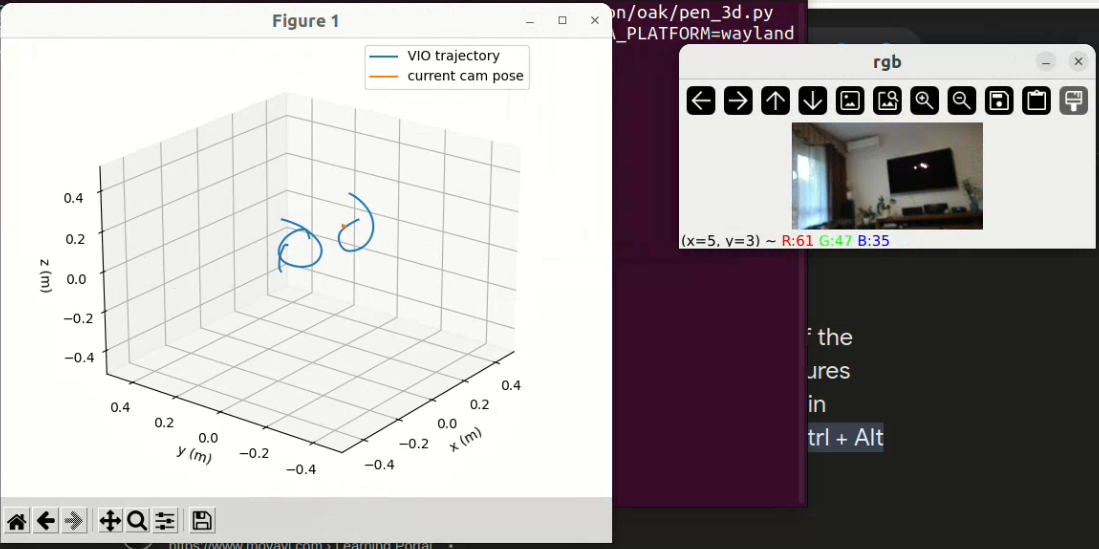
\includegraphics[width=150mm, keepaspectratio]{figures/3d_pen.png}
	\caption{IMU visualization with Spectacular AI}
	\label{fig:3d_pen}
\end{figure}

These examples just visualized the camera's movement and the picture taken with the camera so we did not see any mapping or person detection yet. The repository fortunately provides some spectacular examples on these applications too. However these examples always raised an error which has to be debugged. These examples use OpenGL for visualization and the problem stood in some deep OpenGL code. The easiest way to solve this problem was to comment out some code in \verb|OpenGL/contexdata.py|:

\begin{lstlisting}[language=python,frame=single,float=!ht]
def getContext( context = None ):
    """Get the context (if passed, just return)
    context -- the context ID, if None, the current context
    """
    if context is None:
        context = platform.GetCurrentContext()
    # if context == 0:
        # from OpenGL import errorS
        # raise error.Error(
        # """Attempt to retrieve context when no valid context"""
        # )
    return context
\end{lstlisting}

I understand that it is not the best approach for handling an error like this but it was the least time consuming solution.

Once we digested my absolutely wonderful problem solving technique, we can continue with the examples. We can try out some mapping applications, such as:
\begin{itemize}
    \item point cloud mapping (Figure \ref{fig:SPAI_mapping}),
    \item real-time AR mapping with mesh (Figure \ref{fig:SPAI_mesh_mapping}),
    \item real-time AR mapping with point cloud (Figure \ref{fig:SPAI_point_cloud_mapping}),
    \item mapping with ROS2 integration (Figure \ref{fig:SPAI_ros_mapping}).
\end{itemize}

\begin{figure}[H]
	\centering
	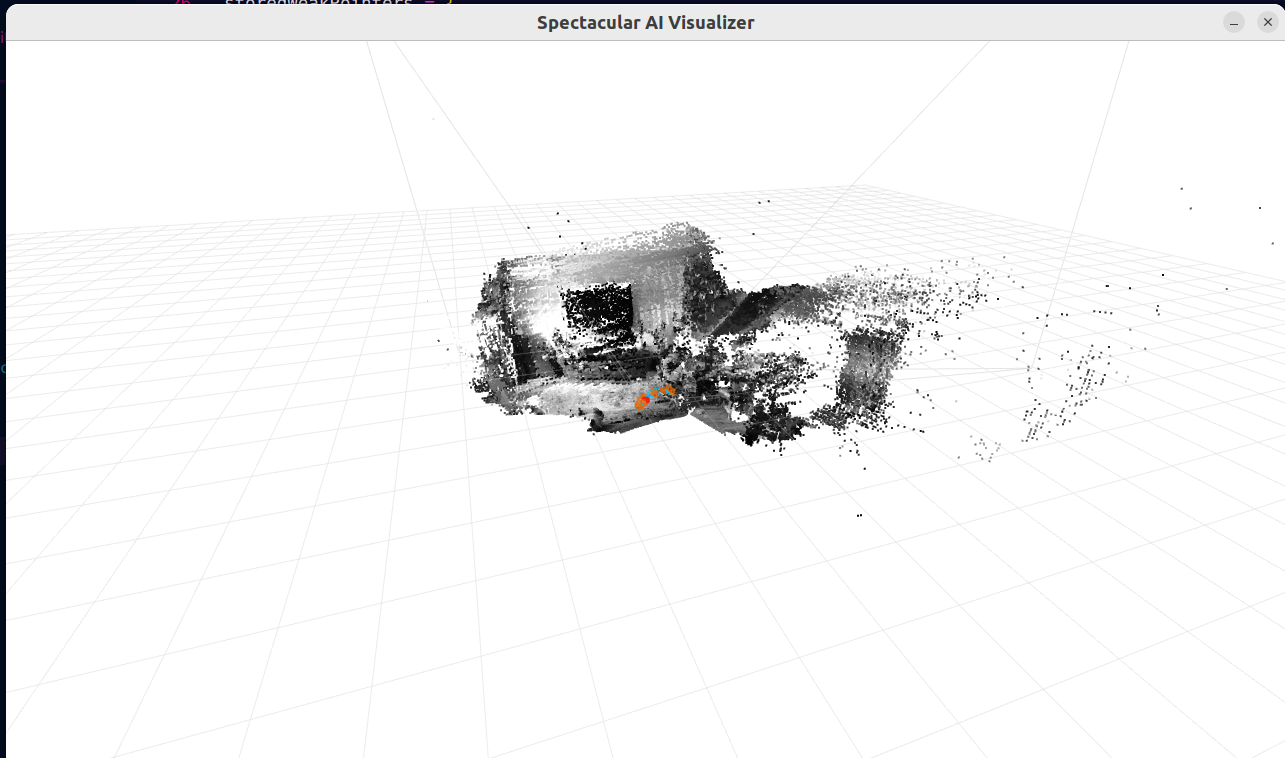
\includegraphics[width=150mm, keepaspectratio]{figures/spectacular_ai_mapping_visu.png}
	\caption{Mapping with Spectacular AI}
	\label{fig:SPAI_mapping}
\end{figure}

\begin{figure}[H]
	\centering
	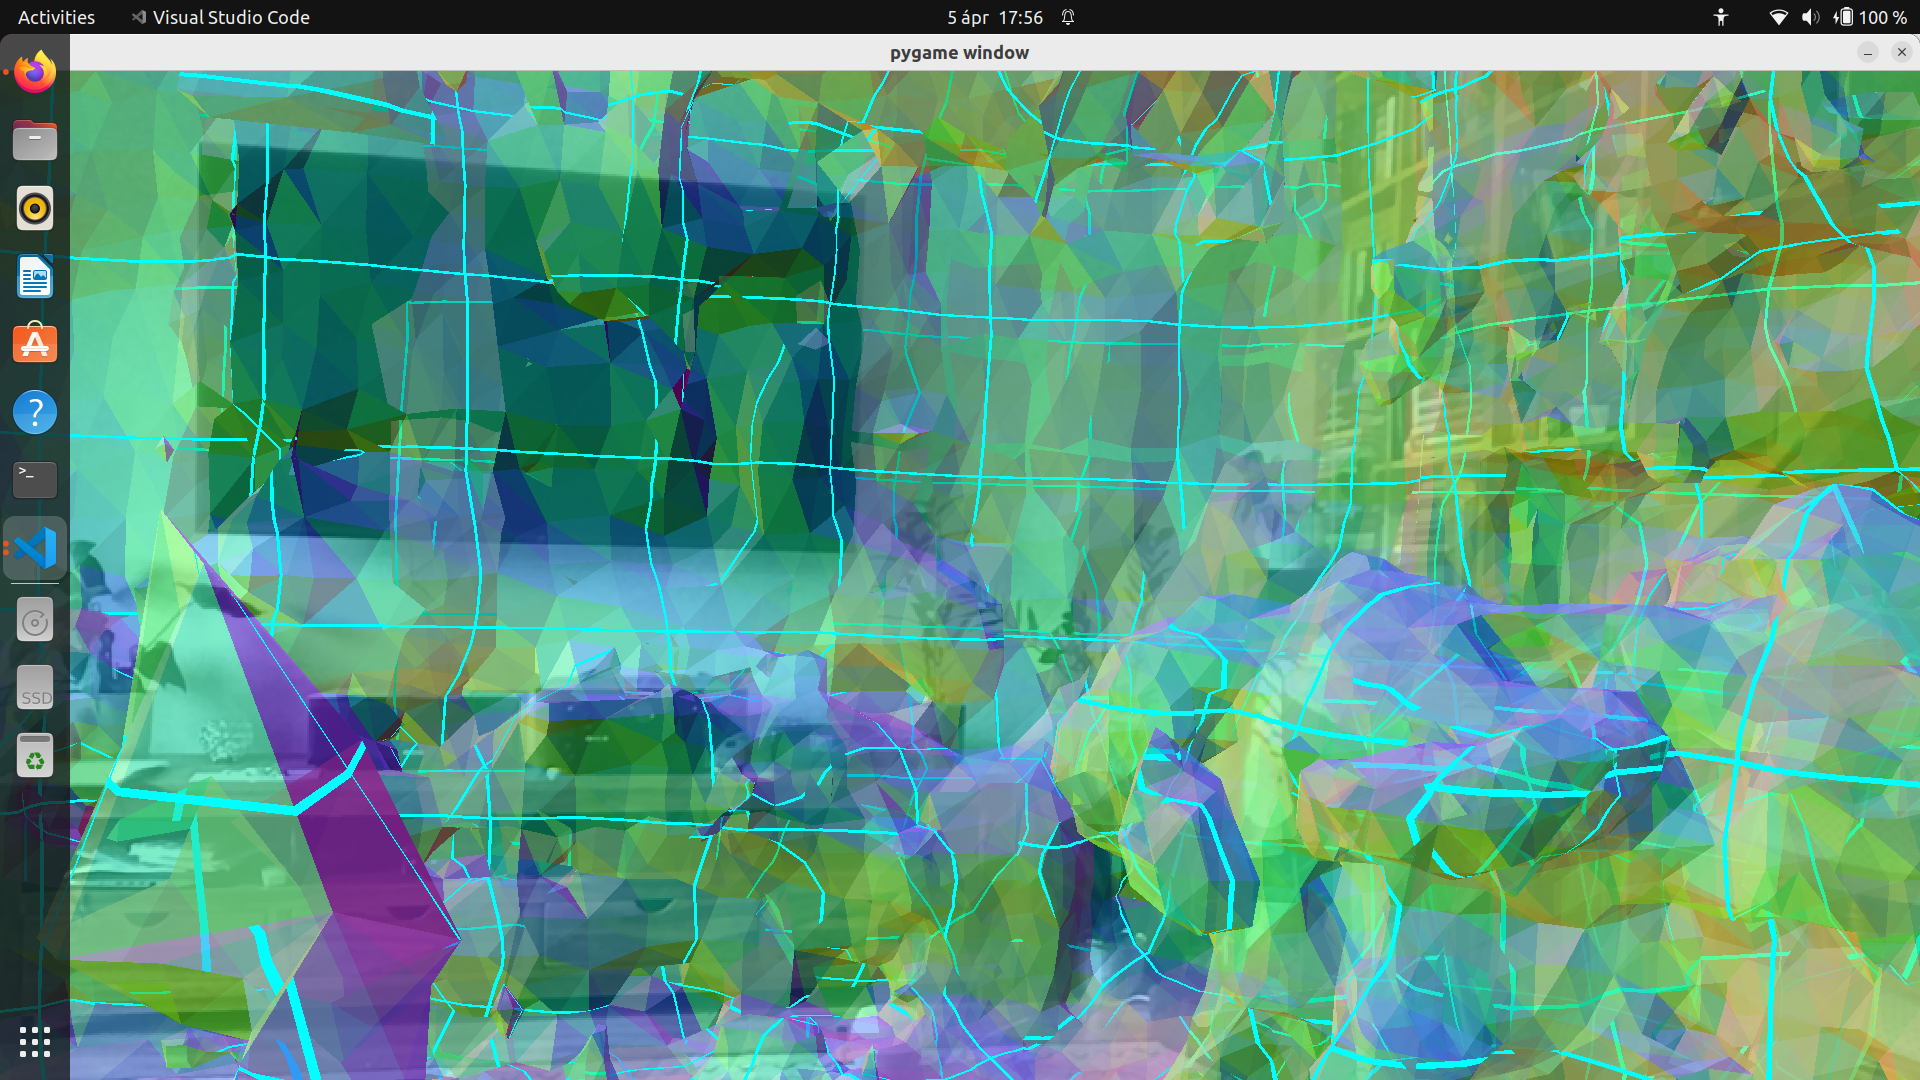
\includegraphics[width=67mm, keepaspectratio]{figures/spectacular_ai_mapping_ar_mesh1.png}\hspace{1cm}
	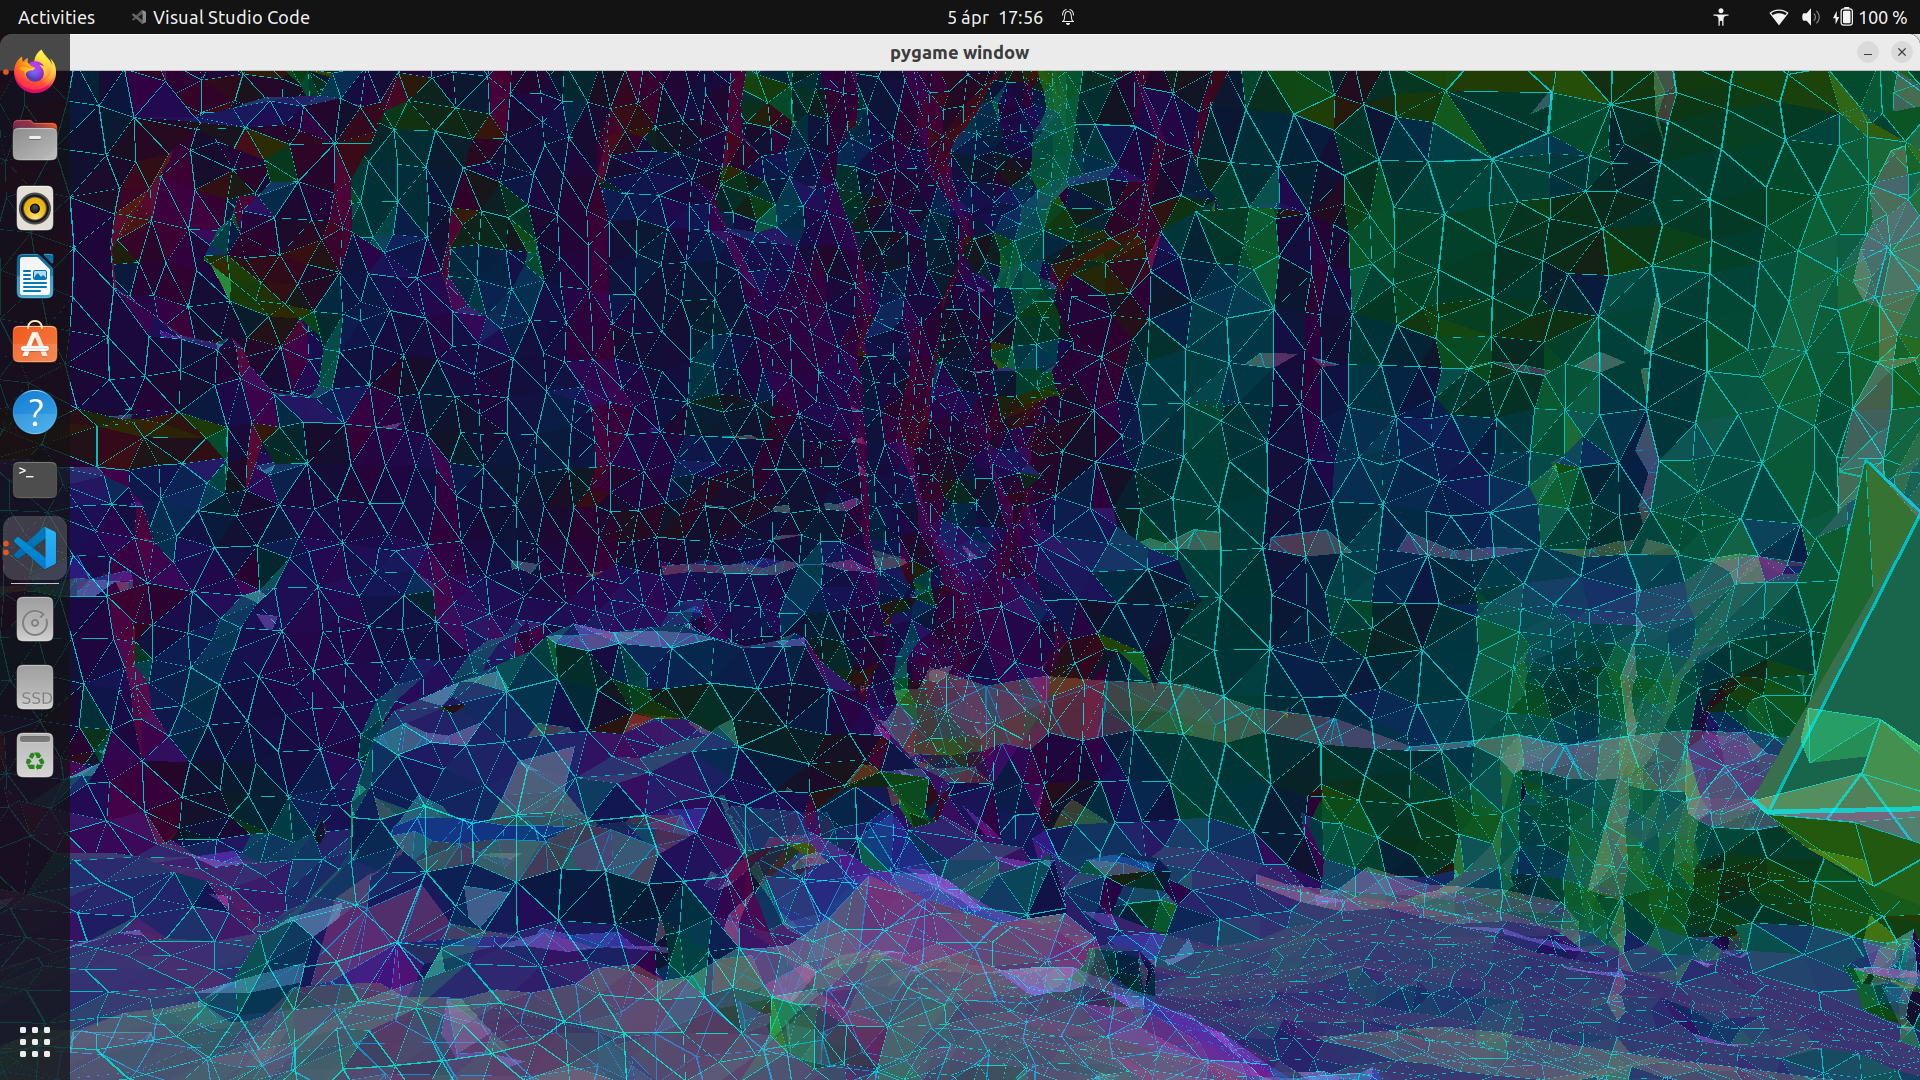
\includegraphics[width=67mm, keepaspectratio]{figures/spectacular_ai_mapping_ar_mesh2.png}\\\vspace{5mm}
	\caption{AR mesh mapping with Spectacular AI}
    \label{fig:SPAI_mesh_mapping}
\end{figure}

\begin{figure}[H]
	\centering
	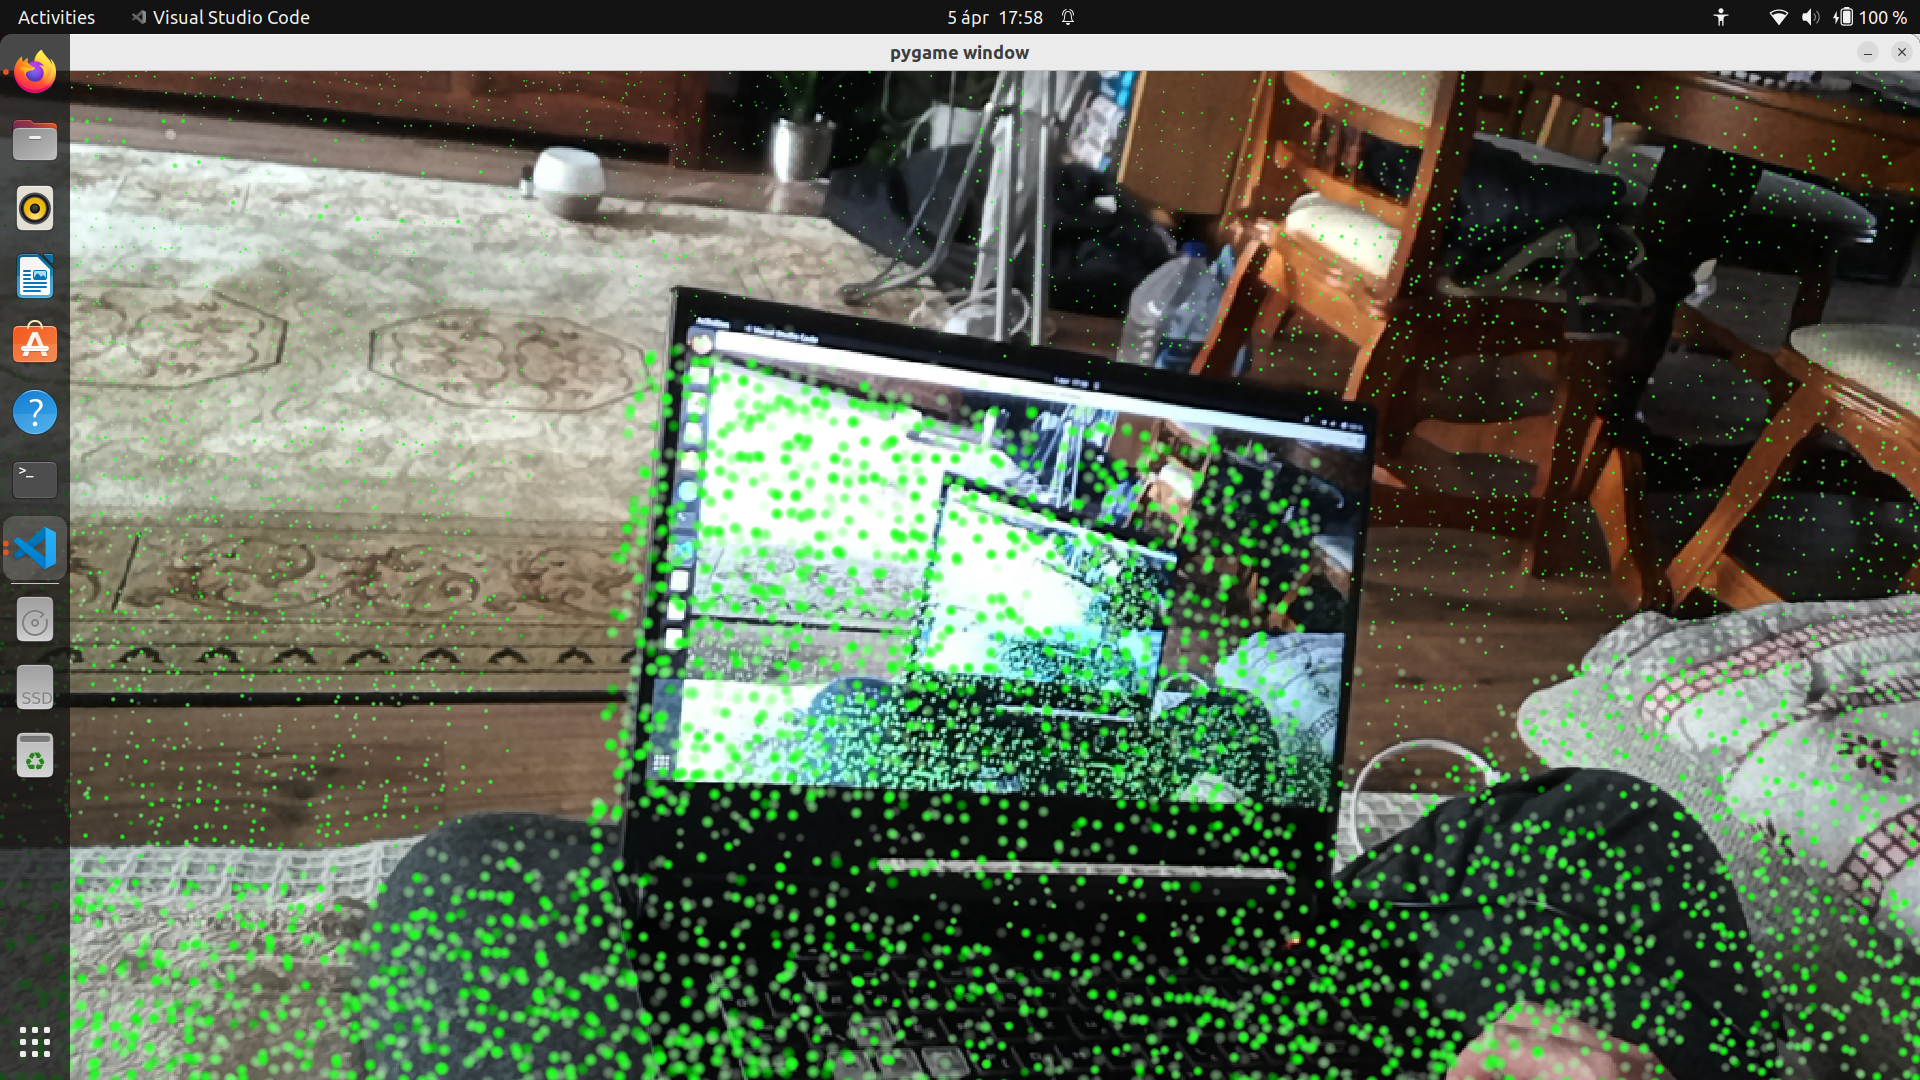
\includegraphics[width=67mm, keepaspectratio]{figures/spectacular_ai_mapping_ar_pc1.png}\hspace{1cm}
	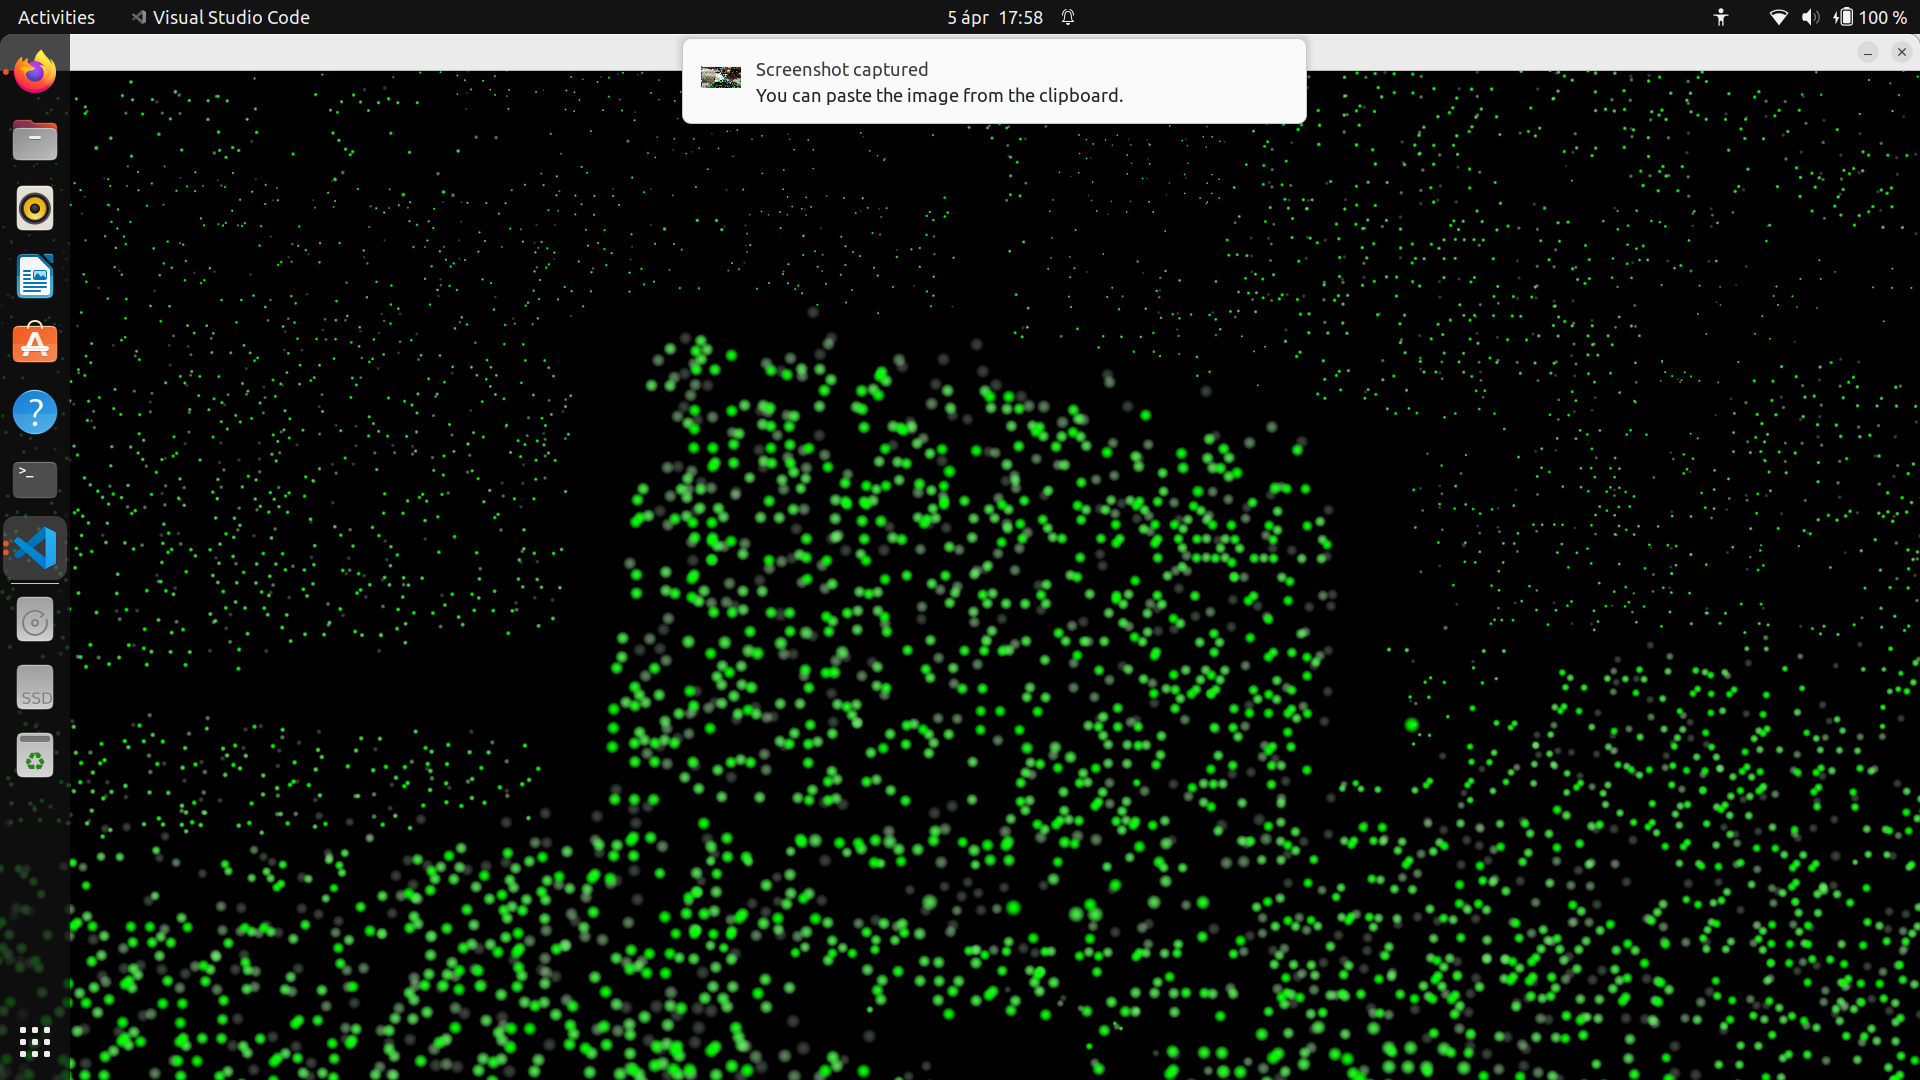
\includegraphics[width=67mm, keepaspectratio]{figures/spectacular_ai_mapping_ar_pc2.png}\\\vspace{5mm}
	\caption{AR point cloud mapping with Spectacular AI}
    \label{fig:SPAI_point_cloud_mapping}
\end{figure}

\begin{figure}[H]
	\centering
	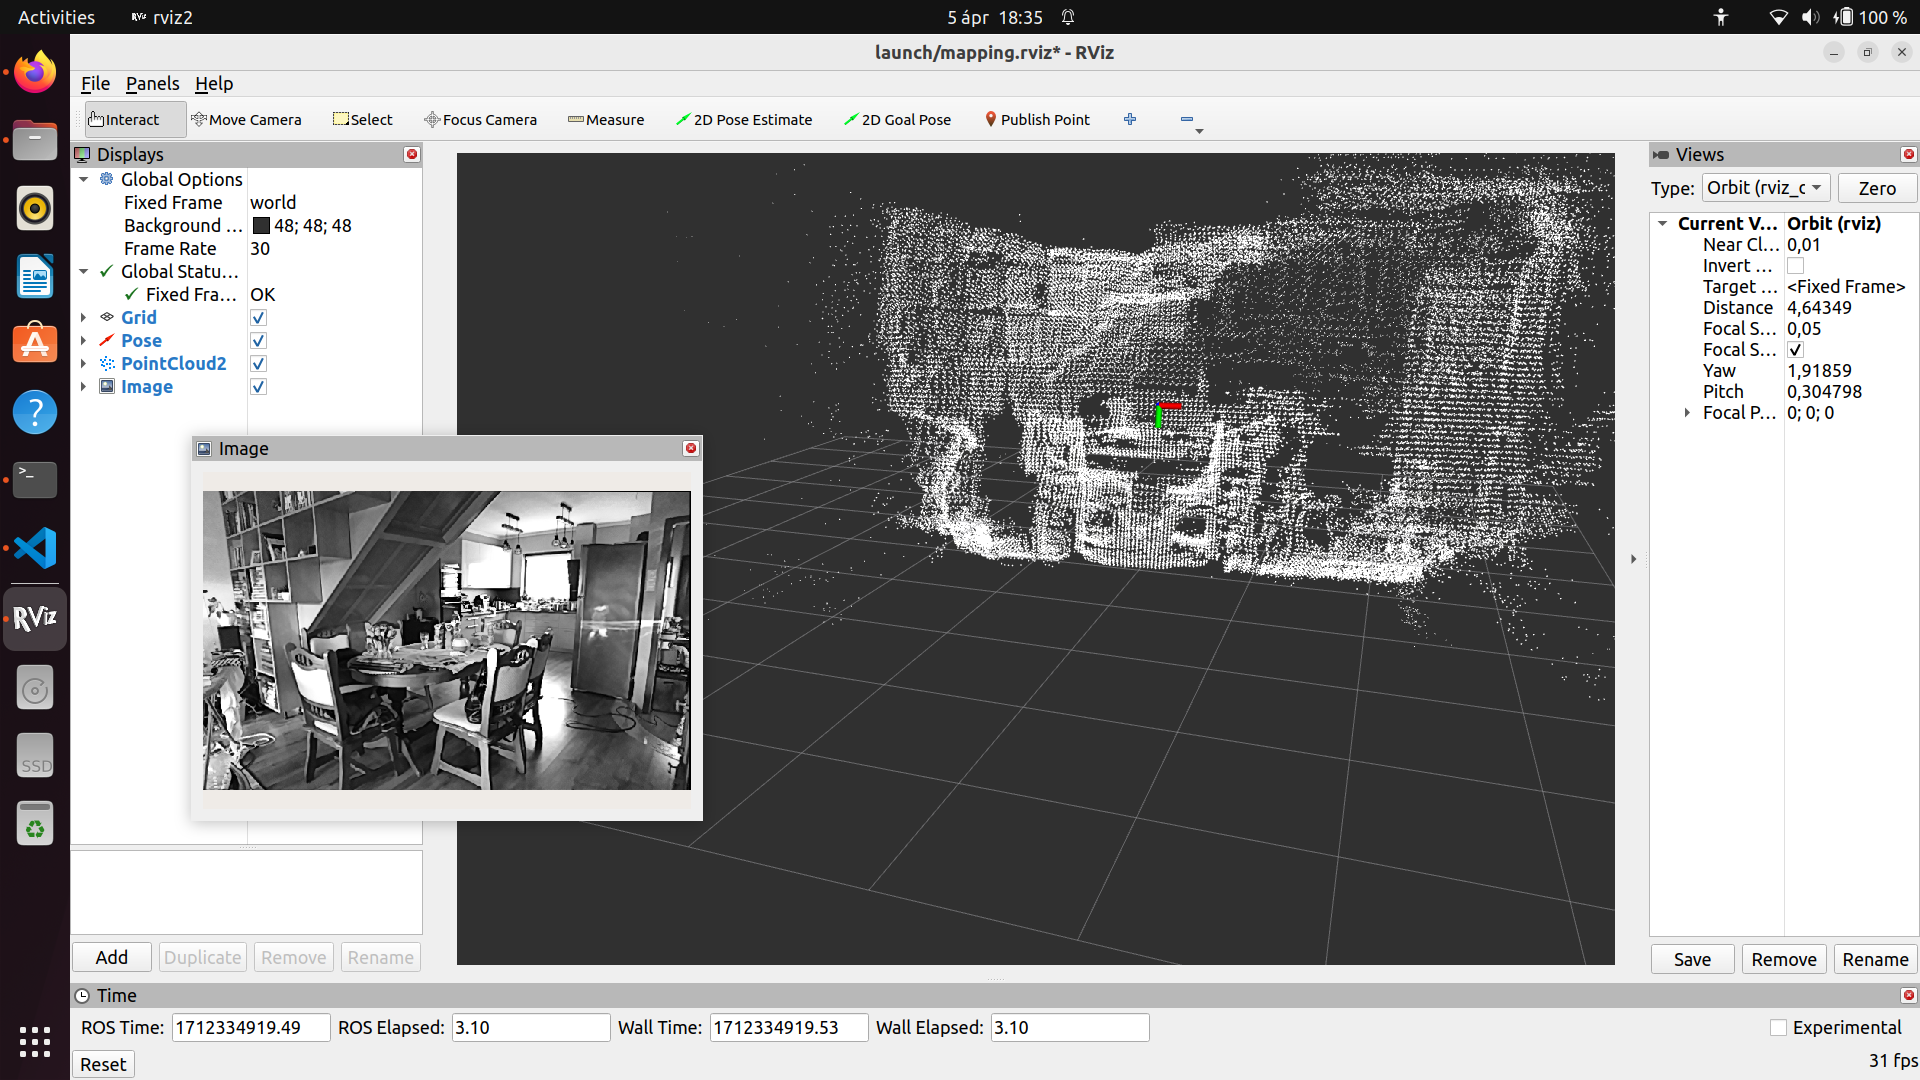
\includegraphics[width=150mm, keepaspectratio]{figures/spectacular_ai_mapping_ros2.png}
	\caption{ROS2 mapping with Spectacular AI}
	\label{fig:SPAI_ros_mapping}
\end{figure}

As we can see the Spectacular AI SDK works really well with the OAK camera. During the testing of the examples I could not experience any major latencies so we can safely say that it works real-time.

I saved the most exciting example for the last one of each. As I said earlier the camera contains a VPU (Intel Movidius Myriad X\footnote{\url{https://www.intel.com/content/www/us/en/products/sku/204770/intel-movidius-myriad-x-vision-processing-unit-0gb/specifications.html}}) which can run neural network models. We do not have to make any post-processing or post-detecting with neural networks because it can be ran on the camera itself. Thanks to the stereo cameras and the VPU OAK is able to detect objects and calculate their location on-the-fly. To select what type of objects we want to detect we have to modify the example code (we only have to modify one list). As we can see on Figure \ref{fig:SPAI_depthai}, I customised the code to detect potted plants in the living room. Due to inadequate lighting the detections did not perform 100\% but they are absolutely acceptable. Moreover I measured the positions of the plants myself and I can safely say that the camera calculated the distances really accurately.

\begin{figure}[H]
	\centering
	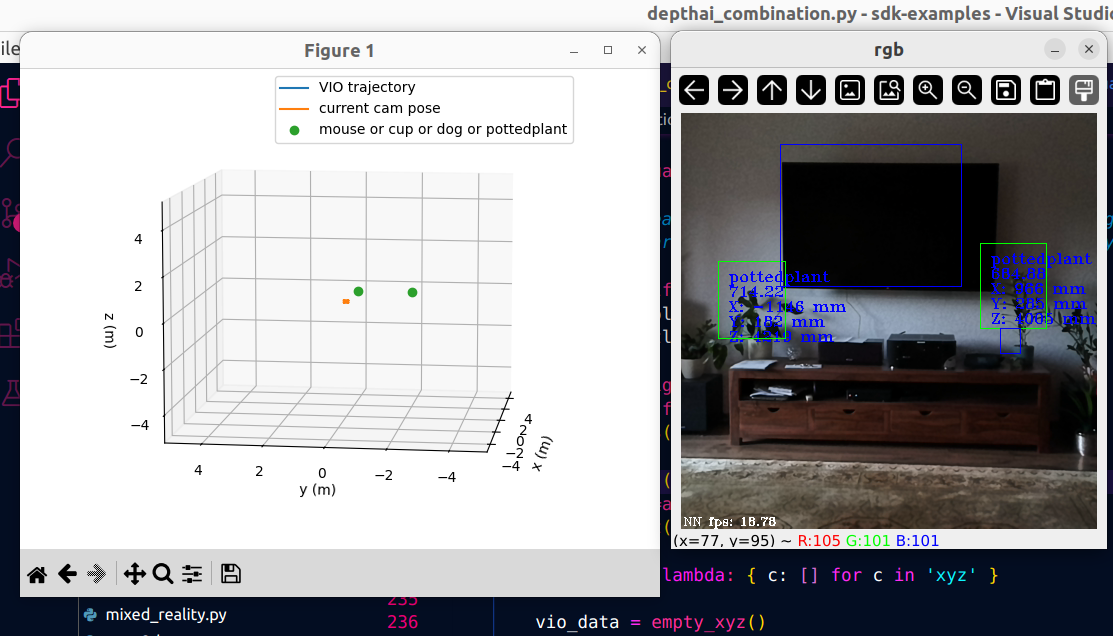
\includegraphics[width=150mm, keepaspectratio]{figures/spectacular_ai_depthai_combination.png}
	\caption{Spectacular AI's object detection and position calculation}
	\label{fig:SPAI_depthai}
\end{figure}

\subsection{RTabMap and person detection}

After experimenting with the camera's examples we continued our journey in the world of mapping. Since the Turtlebot4 is running ROS2 I needed to find a tool that can do the mapping and runs on the said framework.

\section{NeRFs and Gaussian Splatting}

As previously discussed, an additional objective we pursued was to generate 3D photorealistic models of the robot's environment, leveraging images captured during the mapping process. Upon completion of mapping, our aim was to seamlessly integrate the robot's 3D model into this reconstructed scene. This integration would enable real-time simulation of the robot's movements during localization, transcending beyond a mere representation with a point cloud to deliver a highly realistic simulation experience.

Continuing my exploration, I delved into the realm of 3D reconstruction using Neural Radiance Fields (NeRFs)\cite{nerf}. To initiate this process, I utilized an example provided by the Spectacular AI SDK, specifically the \verb|mapping_visu.py| script. This script facilitated the creation of a mapping video, allowing for the specification of an output folder to store both the captured videos from the camera(s) and the resulting point cloud.

\begin{lstlisting}[language=bash,frame=single,float=!ht]
$ python3 mapping_visu.py --recordingFolder /PATH/TO/FOLDER
\end{lstlisting}

We've made significant progress, now possessing videos and a point cloud. However, these resources alone don't suffice as input for NeRFs, which demand a more specific format. NeRFs require not only the images captured at keyframes but also a COLMAP, which contains essential information about the camera setup.

Keyframes serve as pivotal snapshots within the video sequence, capturing unique elements from various perspectives. These frames are crucial for determining the precise position and orientation of the camera at different points in the scene. Drawing a parallel from the animation realm\cite{keyframes_in_animation}, keyframes are akin to markers that delineate significant moments or transitions between actions. In our context, these actions translate to movements such as forward progression or changes in direction.

Additionally, the COLMAP plays a pivotal role by providing foundational data about the camera configuration, including camera positions within each image and a point cloud derived from the scene mapping process\cite{colmap}. This comprehensive dataset serves as the backbone for NeRFs, enabling them to synthesize realistic renderings by leveraging both visual information and spatial context.

By integrating keyframes and COLMAP data, we can create a robust input pipeline for NeRFs, facilitating the generation of immersive and accurate 3D reconstructions from our captured videos and point cloud.

The long-discussed conversion can be done with the help of another Spectacular AI tool, called \verb|sai-cli|. It is a command line tool that can capture videos from OAK cameras and can execute the conversion for NeRF inputs. The required command for creating the input dataset for NeRFs is as follows:

\begin{lstlisting}[language=bash,frame=single,float=!ht]
$ sai-cli process --format FORMAT --preview --preview3d INPUT OUTPUT
\end{lstlisting}

The execution of the command can be observed on Figure \ref{fig:sai_cli_process}. 

\begin{figure}[H]
	\centering
	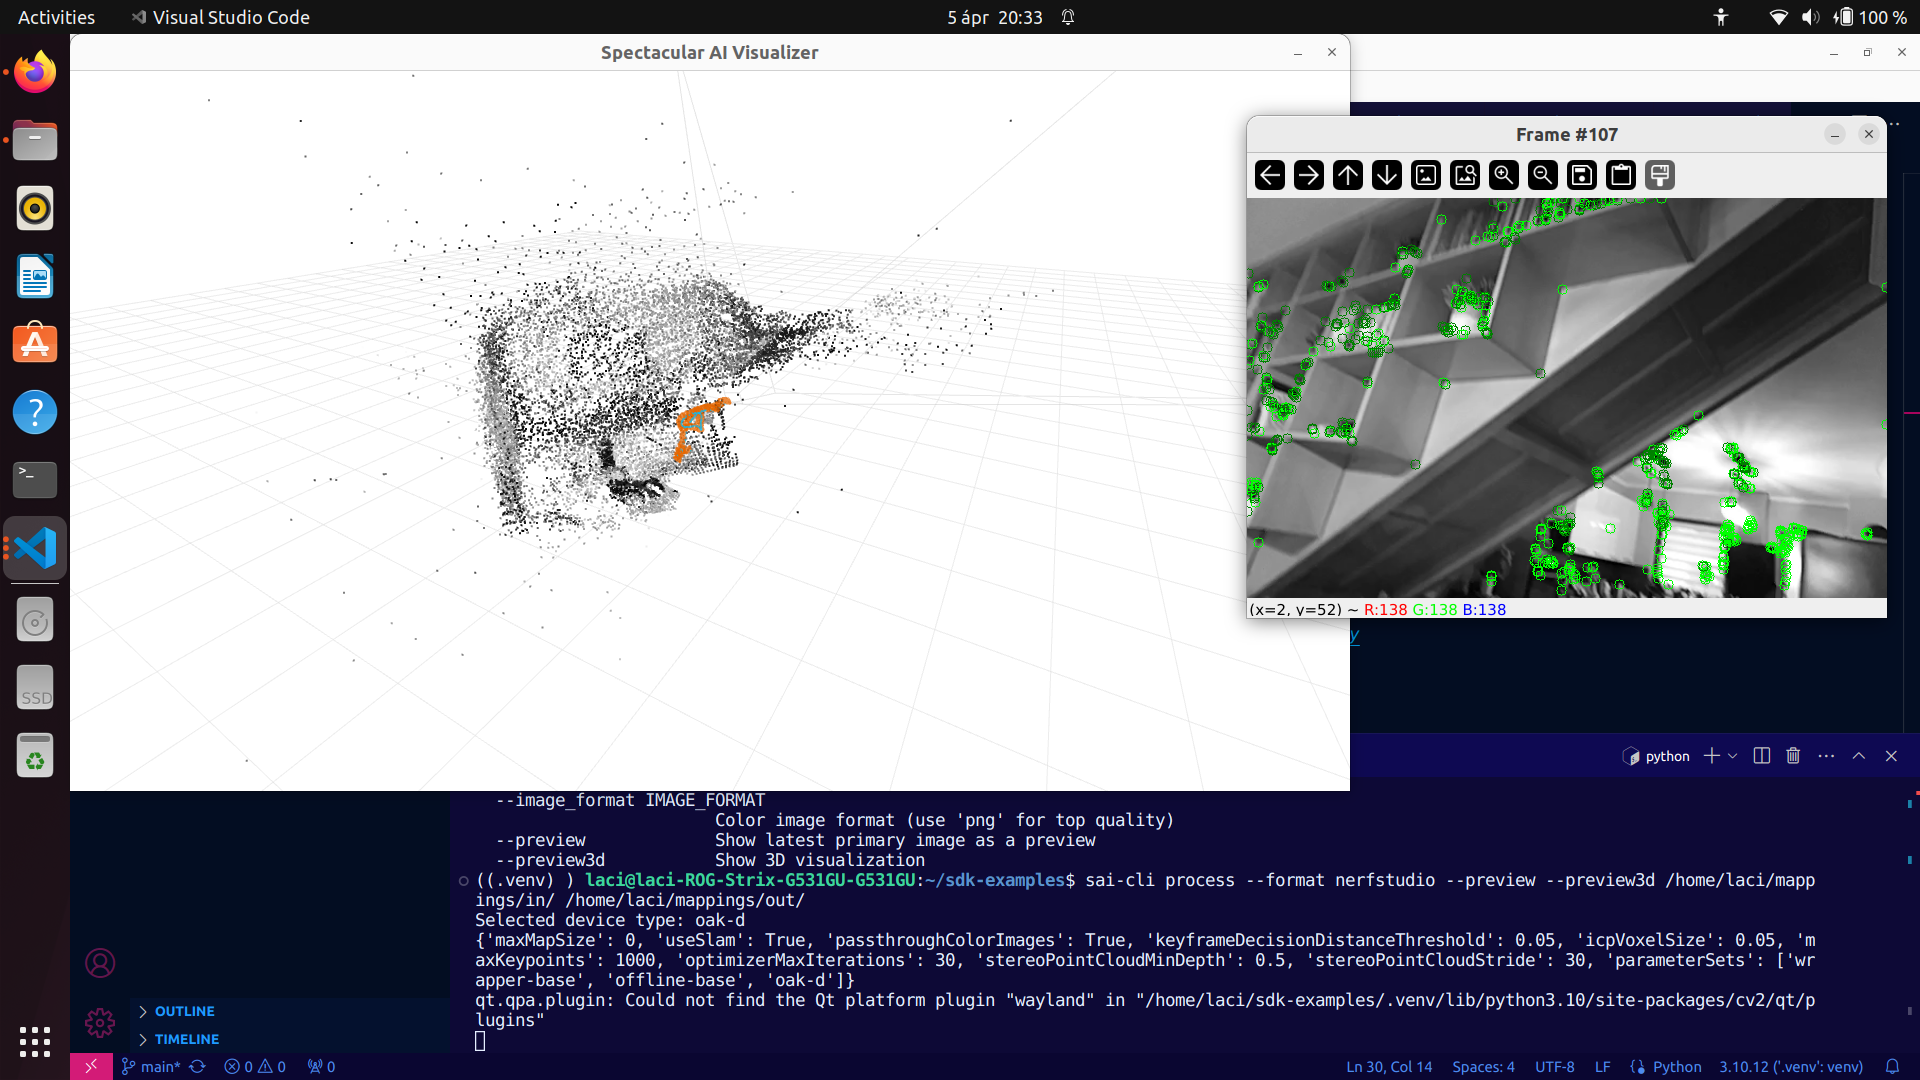
\includegraphics[width=150mm, keepaspectratio]{figures/sai-cli_process.png}
	\caption{Spectacular AI's CLI tool for creating input for NeRFs}
	\label{fig:sai_cli_process}
\end{figure}

With the created input the only thing that stops us from training a NeRF is installing a tool for it. For training I used Nerfstudio\cite{nerfstudio} but due to constant errors during installation with conda I switched to a simpler solution: Docker\footnote{\url{https://www.docker.com/}}. While browsing through the Docker images on DockerHub\footnote{\url{https://hub.docker.com/}}, I experienced that the official Docker image of nerfstudio (nerfstudio/nerfstudio\footnote{\url{https://hub.docker.com/r/nerfstudio/nerfstudio}}) is badly maintained: it is rarely updated and the tagging is unacceptable (the only tag of the image is \verb|latest| so we are unable to pull earlier versions of it)... Thankfully I found a more well-maintained image (dromni/nerfstudio\footnote{\url{https://hub.docker.com/r/dromni/nerfstudio}}) which is updated regularly and tagged professionally.

The Docker container can be started with the following command (I mounted the folders containing the inputs, gave permission for the container to use GPU, specified the user and increased the shared memory which the container can use):

\begin{lstlisting}[language=bash,frame=single,float=!ht]
$ sudo docker run --gpus all \
    -u $(id -u) \
    -v /home/laci/mappings/:/workspace/ \
    -v /home/laci/.cache/:/home/user/.cache \
    -p 7007:7007 --rm -it \
    --shm-size=1gb \
    dromni/nerfstudio:main
\end{lstlisting}

The training can be started inside the container with the following command:
\begin{lstlisting}[language=bash,frame=single,float=!ht]
$ ns-train nerfacto --data PATH_TO_DATA
\end{lstlisting}
It is worth mentioning that nerfstudio has many trainable NeRF models, but for the sake of simplicity I sticked with the one mentioned in the quickstart guide\footnote{\url{https://docs.nerf.studio/quickstart/first_nerf.html}}, which is called nerfacto. The training process and a part of the trained model can be seen on Figure \ref{fig:training_nerf_karcag} and Figure \ref{fig:trained_nerf_karcag}.

\begin{figure}[H]
	\centering
	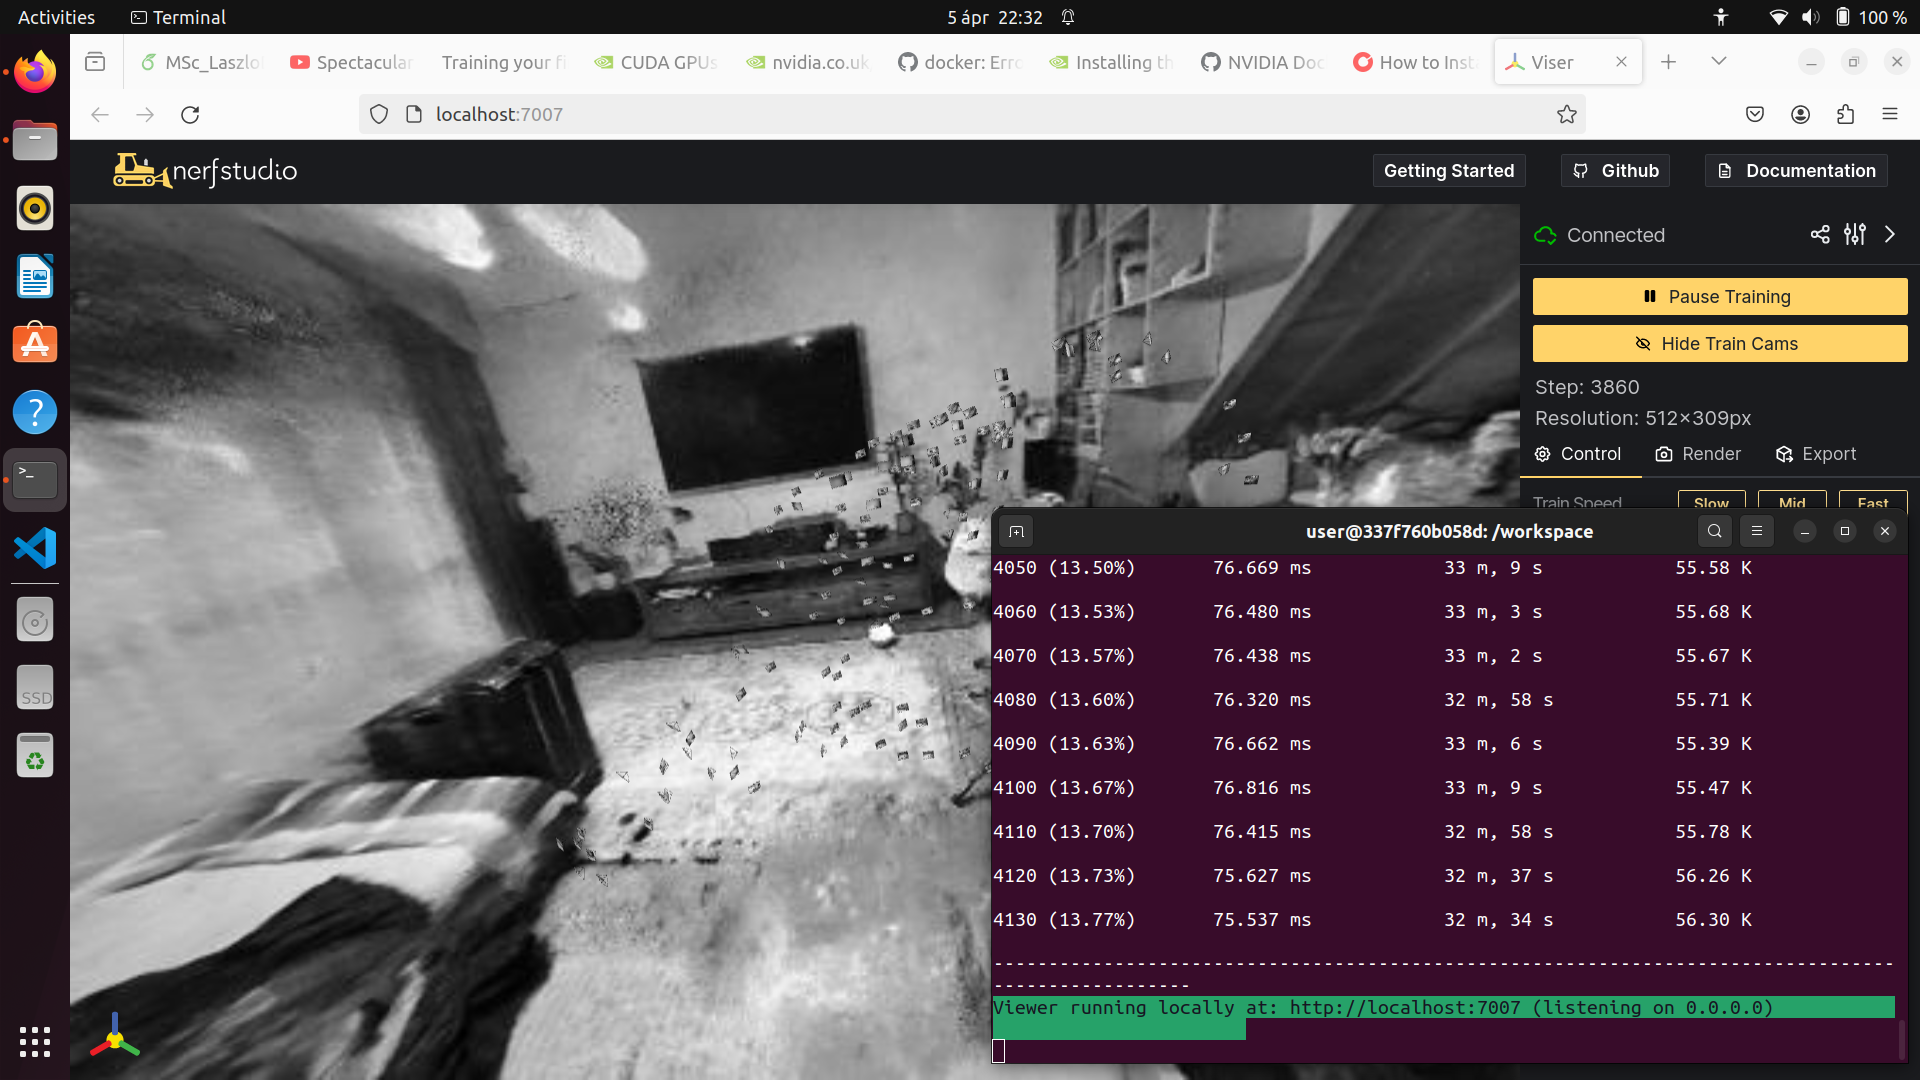
\includegraphics[width=150mm, keepaspectratio]{figures/nerfstudio.png}
	\caption{Training the nerfacto model}
	\label{fig:training_nerf_karcag}
\end{figure}

\begin{figure}[H]
	\centering
	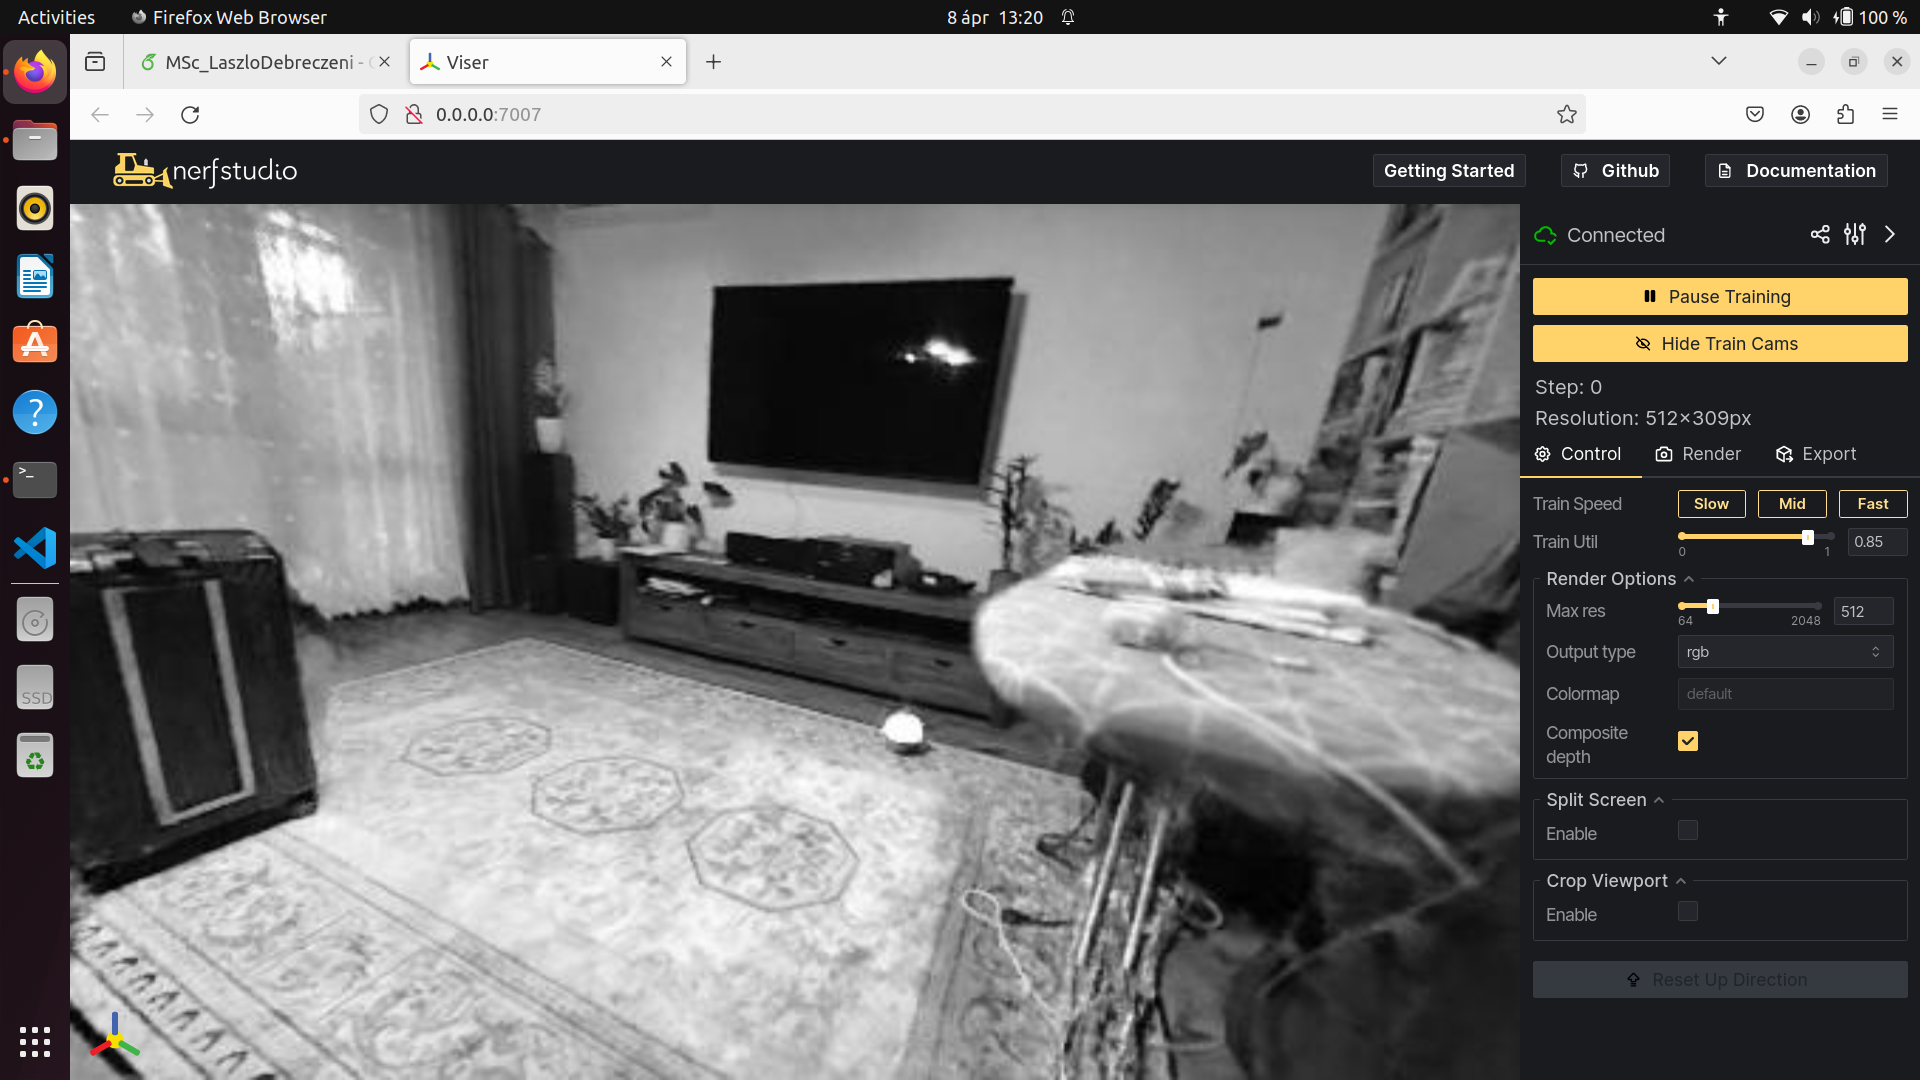
\includegraphics[width=150mm, keepaspectratio]{figures/trained_nerf_karcag1.png}
	\caption{Trained nerfacto model}
	\label{fig:trained_nerf_karcag}
\end{figure}

The result was not without concerns due to the imperfect input:
\begin{itemize}
    \item I captured the video at late afternoon so the lights were on. As seen in Figure \ref{fig:trained_nerf_karcag}, the lights reflected on the TV's screen and some more shiny surfaces causing a significant perturbation in the training.
    \item The other problem was caused by the length of the camera's cable. The device uses an USB3 cable for power and data transport and thanks to this the cable is relatively short for making large scale movements around the laptop connected to it. This resulted in blurry sections in the scene because I was not able to capture every object in the room from every direction.
\end{itemize}

The nerfstudio is capable of generating point clouds from the trained model, we can specify our needs on the viewer which generates us a command that we can run. A point cloud can be seen on Figure \ref{fig:nerfstudio_point_cloud}.

\begin{figure}[H]
	\centering
	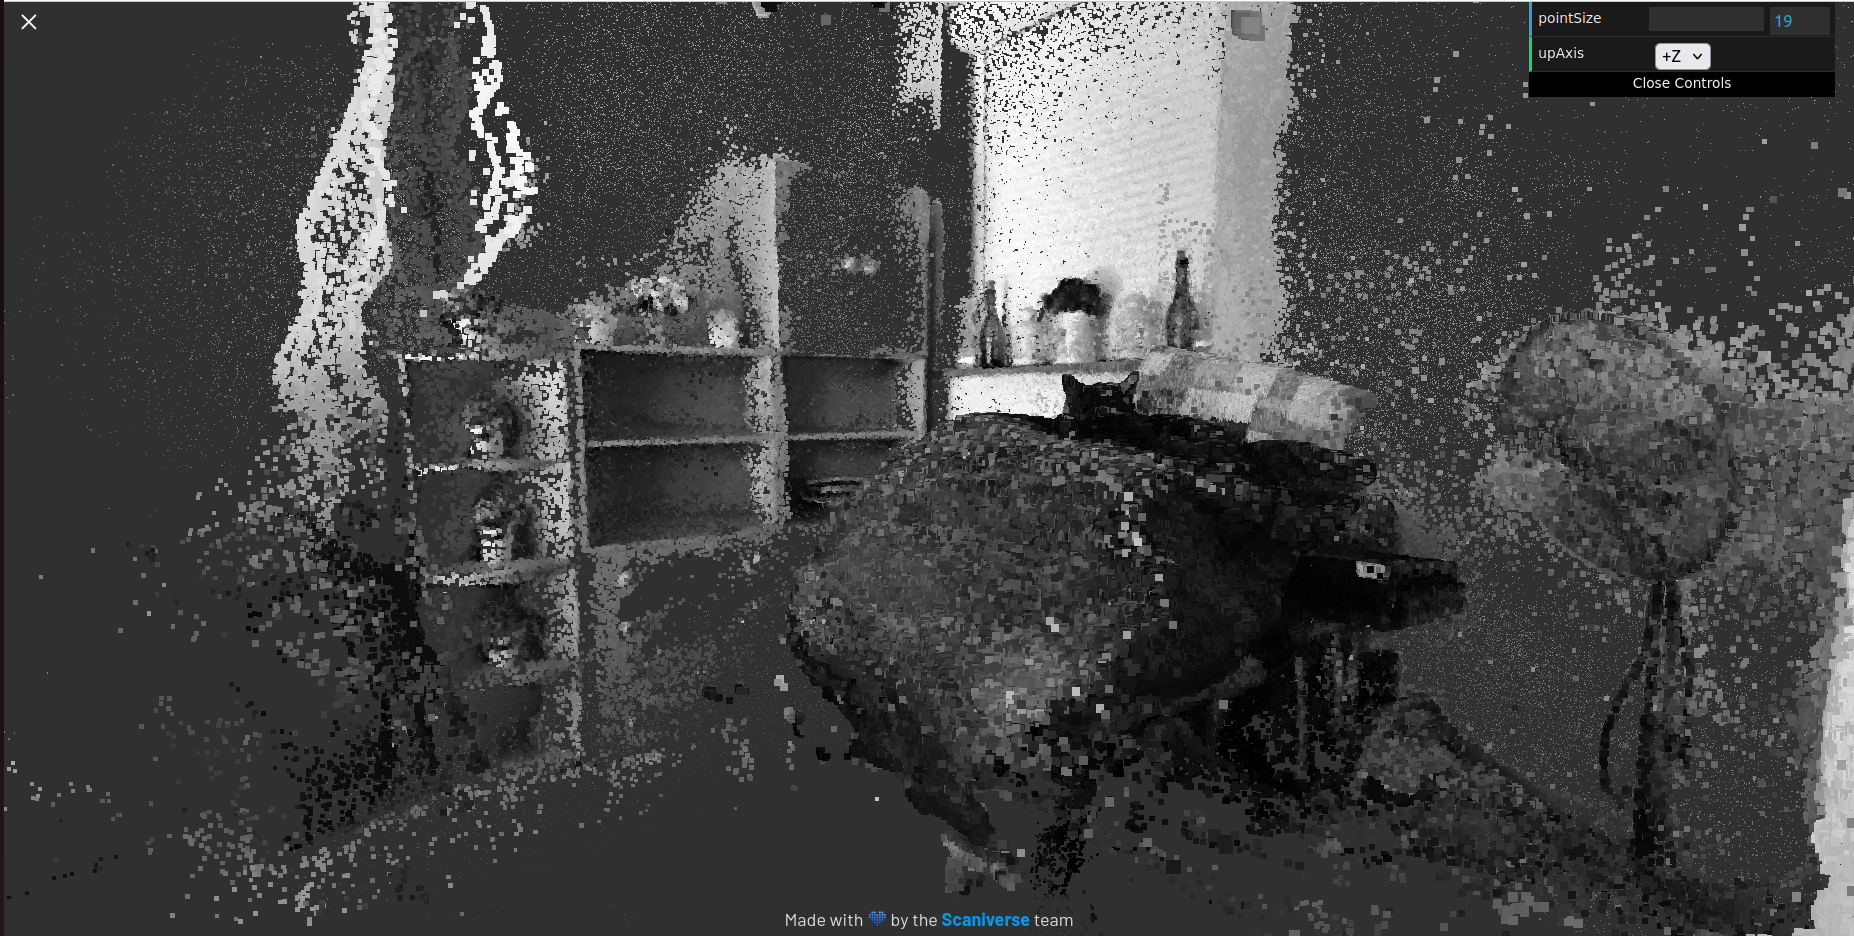
\includegraphics[width=150mm, keepaspectratio]{figures/nerfacto_point_cloud1.png}
	\caption{Point cloud from trained nerfacto model}
	\label{fig:nerfstudio_point_cloud}
\end{figure}

Overall, apart from the errors, a surprisingly good model has been created, thus proving the raison d'être of NeRFs.

We tried out an interesting, more user-friendly method of training NeRFs: Luma AI's iOS application\footnote{\url{https://apps.apple.com/us/app/luma-ai/id1615849914}} (the application exists for Android, too\footnote{\url{https://play.google.com/store/apps/details?id=ai.lumalabs.polar&hl=en_US&pli=1}}). We must own a phone with a LIDAR to use the app, I tried it using an iPhone 13 Pro and it worked absolutely well on it. I captured my cat's (Szotyi's) toy as a test. First I needed to specify the object's dimensions in a modern AR view, then I had to create pictures of the toy in from different angles and positions. The app uploaded the images to the cloud and after some time the NeRF was trained so we could inspect it. The results were truly breathtaking, it was as realistic as the object was right in front of us as seen on Figure \ref{fig:luma_ai_szotyi_toy}

\begin{figure}[H]
	\centering
	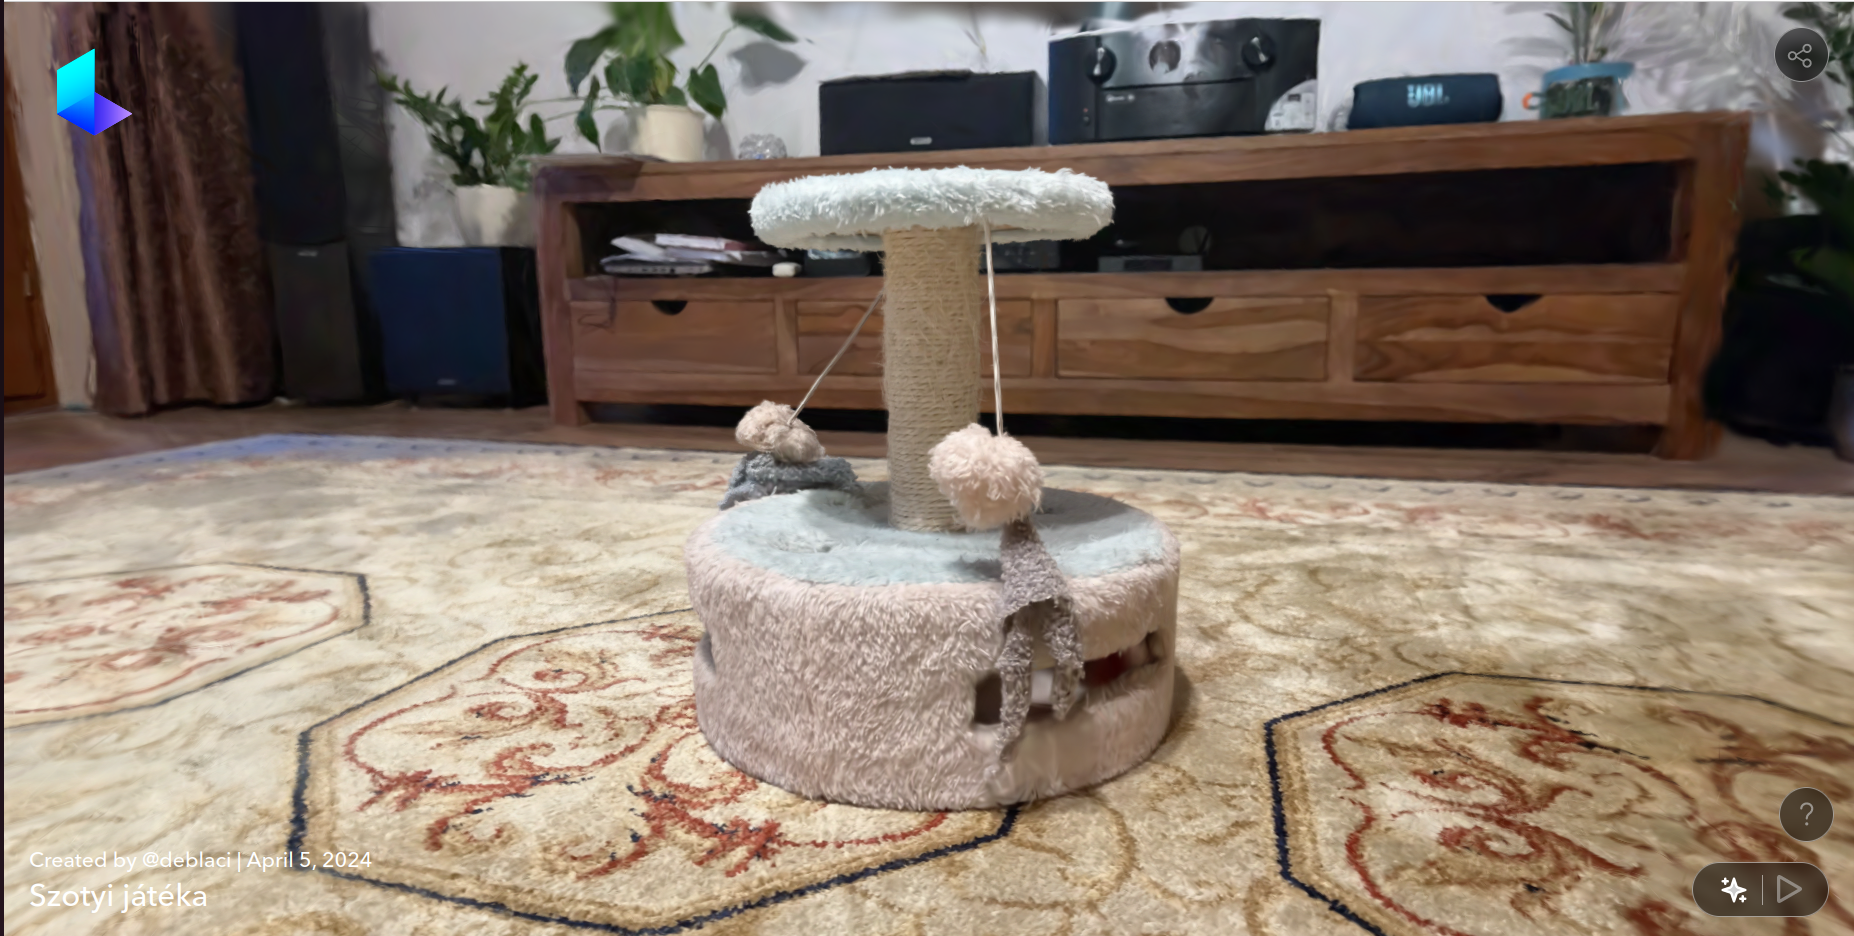
\includegraphics[width=150mm, keepaspectratio]{figures/szotyi_jateka_luma_ai.png}
	\caption{Szotyi's toy recreated by Luma AI}
	\label{fig:luma_ai_szotyi_toy}
\end{figure}

As another approach for photorealistic reconstruction we tried out some Gaussian Splatting\cite{3DGS} implementations. I found out that nerfstudio has a model that uses Gaussian Splatting, this model is called splatfacto\cite{splatfacto} and since I already used nerfstudio I gave it a try. Needless to say it was not without hard parts. As I used the \verb|dromni/nerfstudio| image I always got an error by CUDA because the image did not find it installed (but it was). After some hours of debugging I tried to use the \verb|nerfstudio/nerfstudio| image to see if it works or not. Well, it did not work but I got another error message for the sake of change:

\begin{lstlisting}[language=bash,frame=single,float=!ht]
assert block width > 1 and block width <= 16, 
"block width must be between 2 and 16"
AssertionError: block width must be between 2 and 16
\end{lstlisting}

As I searched for a solution it soon became clear that this is a very low-level problem with either nerfstudio or the splatfacto model\footnote{\url{https://github.com/nerfstudio-project/gsplat/issues/159}}. I tried upgrading the \verb|gsplat| package but the issue remained.

After the failures we tried another Gaussian Splatting\footnote{\url{https://github.com/graphdeco-inria/gaussian-splatting}} which finally started training but it threw \verb|CUDA out of memory| error every time. I inspected the repository and the developers stated that this works with 24 GB of VRAM. I have a GTX1660 GPU in my laptop with 6 GB of VRAM thus it was not enough for training. I tried using Google Colab for training but after it finished it had problems with saving the splats because the command always stopped with Out Of Memory errors and I was left there without the finished splat. My advisor, Gábor tried training on his GTX1080 and fortunately it had enough VRAM to finish it but the result is not worth even an image here because it was too blurry.
